\documentclass{udpreport}
\title{Cableado Estructutado}
\author{Integrantes: Francisca Carrrasco, Ignacio López.\\Profesor: José Pérez
\\Ayudante: Alexis Inzunza}
\date{Abril de 2017}
\usepackage{graphicx}
\graphicspath{ {Imagenes/} }
\udpschool{Escuela de Informática y Telecomunicaciones}

\begin{document}
\maketitle
\tableofcontents
\chapter{Actividades}
	\section{Construcción de un cable directo y un cable cruzado}
	    Para la construcción de ambos cables fueron necesarios los siguientes materiales: 
\begin{itemize}
		\item{\bf Alicate RJ45}
		\item{\bf 2 Trozos de cable de red}
		\item{\bf 4 Cabezales RJ45}
		\begin{figure}[h]
		    \centering
    	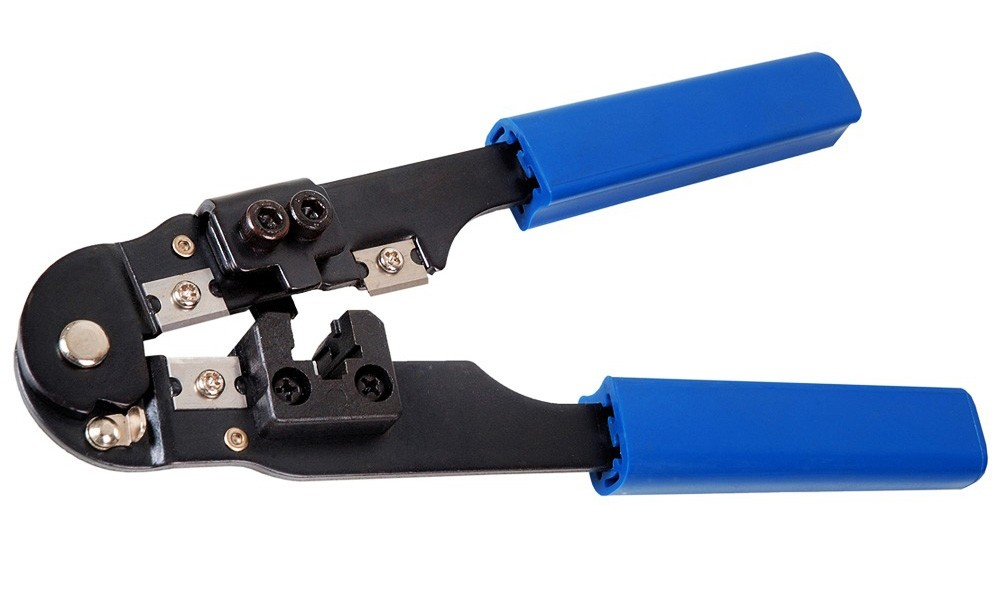
\includegraphics[width=7cm, height=4cm]{alicate.jpg}
    	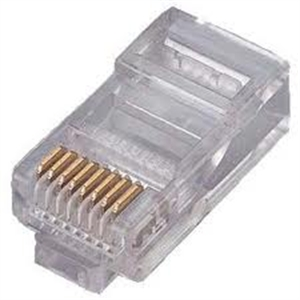
\includegraphics[width=7cm, height=4cm]{cabezal.jpeg}
    	\end{figure}
    	\\Empezando por el cable directo, lo primero que hicimos fue cortar en ambos extremos del cable una parte de su envoltura, para luego poder ordenar las trenzas según la especificación T568-A o T568-B, ambas sirven (nosotros elegimos la T568-A). Una vez ordenados lo siguiente por hacer fue cortar la punta de los pares para que así, al estar del mismo largo pudieran entrar dentro del cabezal RJ45 (hay que verificar que todos los hilos lleguen hasta el fondo), finalmente insertamos el cabezal en el alicate RJ45 (o crimpeador) teniendo cuidado de que no se mueva ningún hilo y lo apretamos para que así quede firme.
    	\\Una vez hecho esto seguimos los mismos pasos para el otro extremo del cable y debemos usar la misma especificación que elegimos anteriormente (de esto depende si el cable que acabamos de construir es un cable directo o cruzado).
    	\\Para hacer un cable cruzado las instrucciones son exactamente las mismas, con la única diferencia de que los pares de ambos extremos deben estar siguiendo distintas especificaciones, es decir, un extremo debe seguir la especificación T568-A y el otro la T568-B.
\end{itemize}
	\section{Cuestionario e Investigación}
		Para esta actividad abrimos un terminal y ejecutamos el comando ``ifconfig'' y se desplegó lo siguiente:\\
		\begin{figure}[h]
    		\centering
    	\includegraphics[width=\textwidth]{blodos.PNG}
		\end{figure}
		Si observamos la imagen lo que está encerrado en un rectángulo rojo representa la MAC del equipo y lo encerrado en un
		rectángulo morado representa la IP del mismo.
\chapter{Conclusión}
    Con la realización de este laboratorio e informe entendimos la importancia de saber cuales son lo usos que posee cada tipo de cable y lo relevante que es tener en cuenta la categoría del mismo, puesto que con estos conocimientos se puede tomar la mejor decisión a la hora de tener diseñar un cableado estructurado como por ejemplo para implementar una LAN, tambíen pudimos conocer los estándares que se utilizan en el cableado estructurado, incluyendo sus utilidades y funciones.
\begin{thebibliography}{x}

\bibitem{mac} \textsc{Mac Vendors},
\textit{http://www.macvendors.com/}

\bibitem{hp} \textsc{HP},
\textit{http://www8.hp.com/cl/es/products/desktops/product-detail.html?oid=7485168}

\bibitem{cisco} \textsc{Cisco},
\textit{http://www.cisco.com/c/en/us/support/switches/catalyst-2960-24tt-l-switch/model.html}

\bibitem{blueline} \textsc{Blue Line},
\textit{http://www.blue-line.es/index.php/cobre/cat5-utp/9-cat5eutpcable.html}

\end{thebibliography}
\end{document}
Contact GitHub 
